\chapter{ESTUDO DE CASO}

Esta proposta de implementação foi motivada através de um cenário de instituição de ensino que necessitava de uma otimização na segurança e compartilhamento de seus recursos de TI. Para melhor gerenciamento e manutenção dos arquivos compartilhados e usuários na rede, seria necessária a implantação de um servidor que centralizasse todas essas tarefas.

Após identificada a necessidade desse novo recurso, foi iniciada uma pesquisa para encontrar um software que atendesse os requisitos. O Windows Server em todas as suas versões até hoje lançadas poderia ser a solução, mas é proprietário e o valor de uma licença da versão 2012 \textit{Datacenter} custa, atualmente, em torno de 10 mil reais \cite{SERVER}. O alto valor da licença acaba inviabilizando a utilização da mesma nas instituições  de ensino e em pequenas empresas. 
Para solucionar esse problema da compra de licenças foi criada uma versão livre, o Samba 4, que faz as mesmas tarefas de um Windows Server, trabalhando com o mesmo protocolo, o LDAP. Por ser livre, foi utilizada neste trabalho.
A instituição abordada neste trabalho contém 110 computadores nos setores administrativos e 90 nos laboratórios de informática. Abaixo uma pequena demonstração da estrutura da rede:

\begin{figure}[ht]
   	\centering
    \scalebox{1}{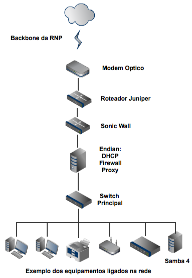
\includegraphics{figuras/iff}}
   	\caption{Estrutura da rede do instituto}
    \label{rede}
\end{figure}
          				
Os setores são divididos conforme suas funções no organograma da instituição. Os principais são:

* Diretoria do Departamento de Administração e Finanças

* Diretoria do Departamento de Gestão de Pessoas

* Coordenação de Registros Acadêmicos

* Chefe de Gabinete

Com a proposta de implementação abordada neste trabalho, cada setor e usuário terá na rede um compartilhamento próprio, com suas permissões definidas. Um servidor foi inserido na rede com o sistema operacional Debian 6.0.5 e com as seguintes configurações:

\begin{itemize}
	\item{Processador Intel Core I7\textregistered}
	\item{4GB de memória RAM}
	\item{Um servidor com 6 Tb de HD}
	\item{Placas de vídeo, áudio e rede Onboard}
\end{itemize}

Antes da instalação do Samba 4 seus pré requisitos foram instalados e o Kerberos Heimdal com suas variáveis de ambiente.
Após a configuração dos sistemas básicos, o Samba 4 foi configurado com os seguintes parâmetros.

\# cd /usr/local/samba/

\# sbin/provision "--use-ntvfs "--realm=instituto.ensino "--domain=instituto "--adminpass= Senha12 "--server-role=’domain controller’

Com o samba 4 as configurações básicas realizadas, foram feitas as modificações necessárias para que fosse utilizado o servidor de dns \textit{default} do samba 4. Foi inserido no domínio do \textit{Active Directory} todas as máquinas Windows XP, através do processo manual e as máquinas Linux, através do script smbad.sh, que se encontram na rede.

Por não ter uma ferramenta mais completa para o gerenciamento do Samba 4 pelo Linux, um computador com Windows XP foi designado para tal tarefa. Nele foram instalados o adminpack e o gerenciador de gpo do Windows. Por trabalharem com o mesmo protocolo como já foi dito anteriormente não houveram incompatibilidades na utilização das ferramentas.

Os usuários foram criados a partir da interface gráfica do adminpack no Windows, respeitando os requisitos de nome completo, ramal da sala, sala, entre outras informações que auxiliam na identificação dos usuários no AD e inseridos nos respectivos grupos dos seus setores.

Com os usuários cadastrados e inseridos em seus grupos, foram criadas as GPO`s com os scripts de inicialização e nelas foram definidos os mapeamentos automáticos dos compartilhamentos

Foram criados compartilhamentos com os nomes dos setores mais importantes da instituição afim de melhorar e garantir o melhor trabalhos das pessoas no setor. Com a intenção de melhorar o controle dos recursos de armazenamento foram impostas regras de QUOTA com o EDQUOTA que consiste em um dos principais programas gerenciadores de cota de disco no linux.

\begin{itemize}
		\item {Pasta do usuário: 20Gb}
		\item {Pasta do setor: 100Gb}
\end{itemize}

A seguir é apresentada uma parte do smb.conf do Samba 4, que corresponde as seções de compartilhamento de arquivos. As seções foram inseridas com a sigla dos setores. Foi decidido vetar arquivos de vídeo e áudio para não sobrecarregar o servidor.

[Chefia\_de\_Gabinete]

comment = Chefia de gabinete

path = /srv/samba/chefia

valid users = +direcao

read only = no

force group = direcao

browseable = no

veto files = *.wmv/*.avi/*.wma/*.mp?/*.flv

[DDAF] 

comment = Diretoria do Departamento de Administração e Finanças

path = /srv/samba/ddaf

valid users = +ddaf

read only = no

force group = ddaf

browseable = no

veto files = *.wmv/*.avi/*.wma/*.mp?/*.flv

[DDGP] 

comment = Diretoria do Departamento de Gestão de Pessoas

path = /srv/samba/ddgp

valid users = +ddgp

read only = no

force group = ddgp

browseable = no

veto files = *.wmv/*.avi/*.wma/*.mp?/*.flv

[CRA] 

comment = Coordenação de Registros Acadêmicos

path = /srv/samba/cra

valid users = +registro

read only = no

force group = registro

browseable = no

veto files = *.wmv/*.avi/*.wma/*.mp?/*.flv


[HOME] 

comment = Pasta dos usuários

path = /srv/samba/\%U

valid users = \%U

read only = no

browseable = no

veto files = *.wmv/*.avi/*.wma/*.mp?/*.flv

Com as sessões criadas no samba, as pastas foram criadas no /srv e atribuídas as permissões 770 com o proprietário root e o grupo com o nome do setor ou do usuário que será designado a pasta:

mkdir /srv/samba/ddgp

chmod 770 -R /srv/samba/ddgp

chown root:ddgp -R /srv/samba/ddgp

Todas as impressoras foram colocadas na rede, mapeadas no servidor do Samba 4 e compartilhadas para os demais computadores com a instalação dos drives automática.

[printers] 

print ok = yes 

guest ok = yes

path = /var/spool/samba 

browseable = yes

[print\$] 

path = /var/lib/samba/printers 

read only = yes

write list = root 

inherit permissions = yes